\section{Introdução}

%------------------------------------------------------
\begin{frame}{Motivação}
\begin{itemize}
    \item Em muitos problemas, não há dificuldade em determinar se um dado elemento é ou não parte de um grupo
    \item $7 \in \mathbb{N}$ e $-7 \notin \mathbb{N}$
    \item Diversos fenômenos na natureza não podem ser classificados com conjuntos clássicos
    \item Relação de pertinência não é bem definida \citep{pedrycz:98}
    \item Incerteza e imprecisão nos conjuntos de dados
    \item Explorar a capacidade de conjuntos \emph{fuzzy} de expressar transições graduais de pertinência e não pertinência
\end{itemize}
\end{frame}

%------------------------------------------------------
\begin{frame}{Motivação}
\begin{figure}[h]
    \centering
    \begin{minipage}{0.48\textwidth}
        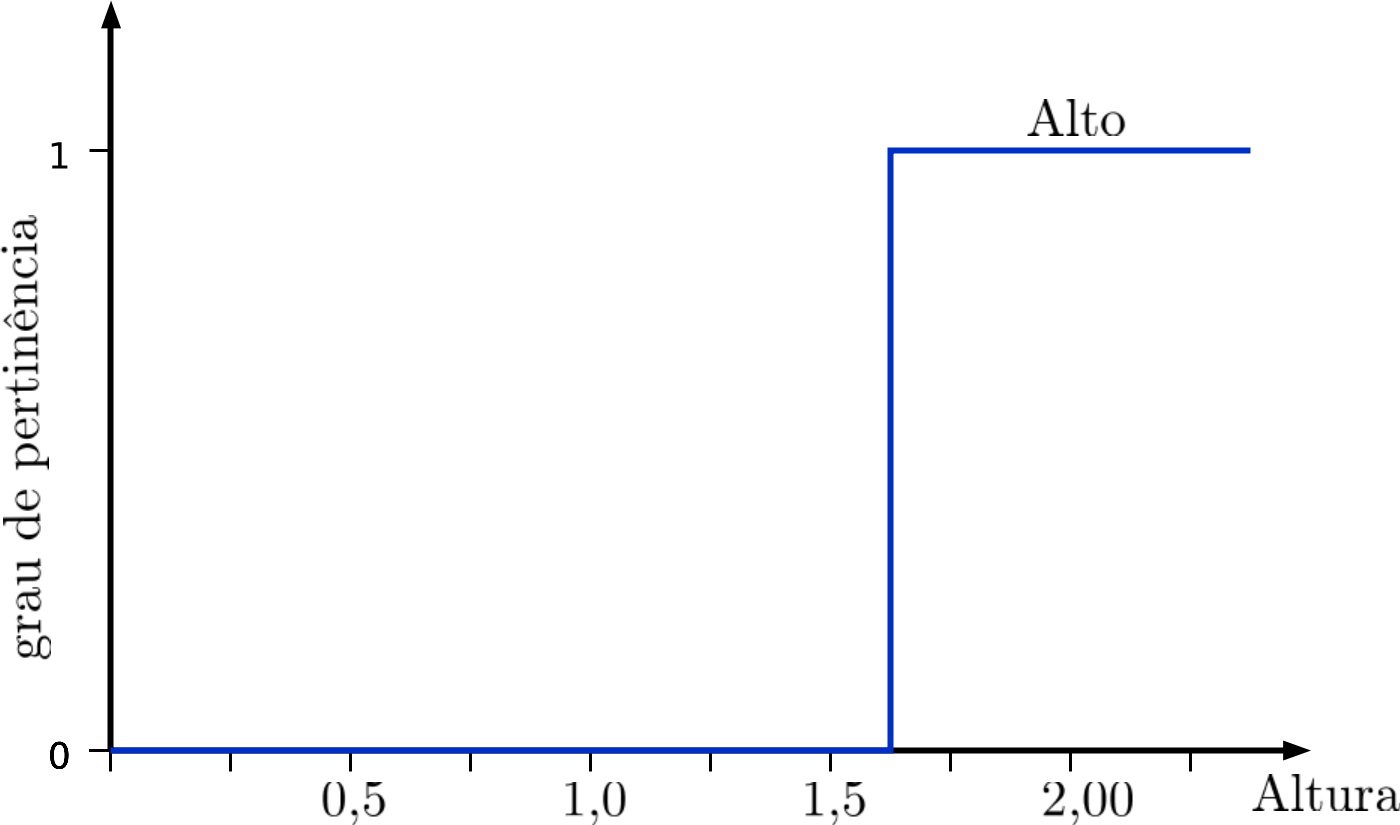
\includegraphics[width=\textwidth]{crisp_set}
    \end{minipage}
    ~ % space
    \begin{minipage}{0.48\textwidth}
        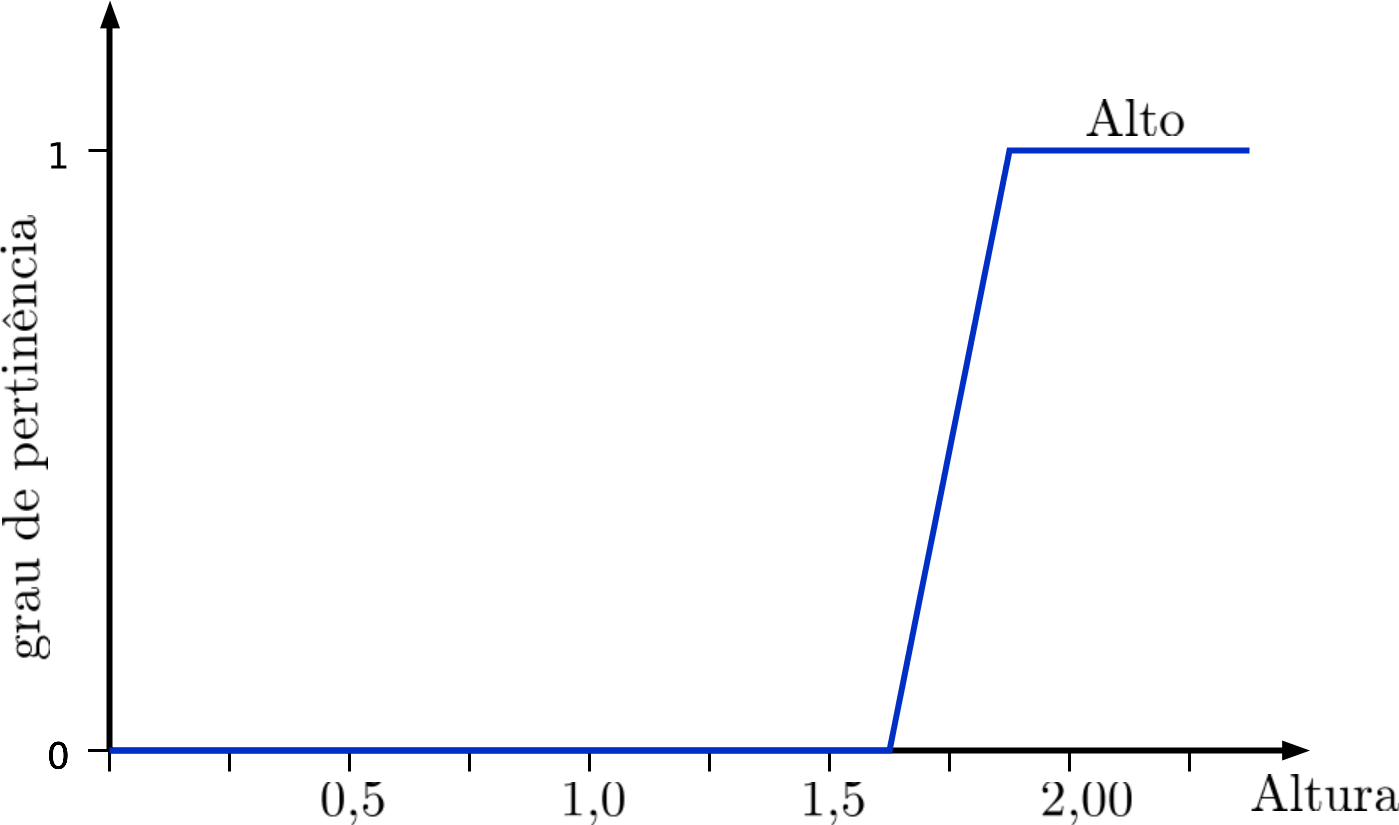
\includegraphics[width=\textwidth]{fuzzy_set}
    \end{minipage}
\end{figure}
\end{frame}

%------------------------------------------------------
\begin{frame}{Trabalhos relacionados}{Classificação com conjuntos \emph{fuzzy}}
\begin{itemize}
    \item Algoritmo de árvore de decisão \emph{fuzzy} \citep{umano:94}, adaptado do ID3 clássico proposto por \citet{quinlan:86}
    \item \citet{bhatt:09} segmentaram regiões de pele no espaço RGB; cinco \emph{clusters} com \emph{fuzzy c-means} \citep{bezdek:84}; taxa de erro obtida 94,1\%
    \item \emph{FuzzyDT} proposta por \citet{cintra:13}, baseado no C4.5 \citep{quinlan:93}
    \item Formulação geral de \emph{kernel} sobre conjuntos \emph{fuzzy} \citep{guevara:14}
\end{itemize}
\end{frame}

%------------------------------------------------------
\begin{frame}{Trabalhos relacionados}{Detectores de pele}
\begin{itemize}
    \item Regra de decisão Bayesiana com um modelo de histograma $3$-dimensional; histogramas de tamanho 32 mostraram o melhor desempenho com uma taxa de erro de 88\% \citep{jones:02}
    \item Classificação com regras no modelo de cores YCbCr; taxa de verdadeiro positivo de 90,66\% \citep{kovac:03}
    \item \citet{yogarajah:11} desenvolveram uma técnica onde os limiares definidos nas regras são adaptados dinamicamente
\end{itemize}
\end{frame}

%------------------------------------------------------
\begin{frame}{Trabalhos relacionados}{Comparação do modelo de cores}
\begin{itemize}
    \item Abordagens Gaussiana e histograma em 805 imagens coloridas em 9 espaços de cores distintos; SCT, HSI e CIELab com abordagem de histograma \citep{jayaram:04}
    \item 10 espaços de cor com base no \emph{k-means} em 15 imagens do AR; YCgCr, YDbDr e \textbf{HSV} \citep{chaves:10}
    \item \citet{kaur:12} similar ao proposto por \citet{kovac:03} com operações morfológicas e de filtragem no YCbCr e \textbf{CIELab}, ignorando o componente de luminância em ambos
    \item Técnica similar implementada em \citet{shaik:15} e \citet{kumar:15} nos espaços de cores HSV e \textbf{YCbCr}
\end{itemize}
\end{frame}

%------------------------------------------------------
\begin{frame}{Objetivos}
\begin{itemize}
    \item Estudo de conjuntos e números \emph{fuzzy}
    \item Modelagem de conjuntos \emph{fuzzy} para classificação
    \item Estudo de classificação \emph{fuzzy}
    \item Escolher uma aplicação real para aplicar a modelagem \emph{fuzzy}
    \item Compreender a influência do espaço de cores para a modelagem dos dados
\end{itemize}
\end{frame}